\subsubsection{Datenbank und Cloudspeicher}\label{datenbank und cloudspeicher}
Die verwendete Datenbank ist ein Firestore von Firebase. Firestore ist ein Cloud NOSQL Datenbanksystem. 
Die Daten werden in sogenannte Kollektionen und Dokumente eingeteilt. 
Dabei gehören zu jeder Kollektion Dokumente, in welchen die eigentlichen Daten gespeichert sind. 
In Abbildung \ref{fig:datenbank_aufbau} ist der Datenbankaufbau zu sehen.
\begin{figure}[h]
 \centering
 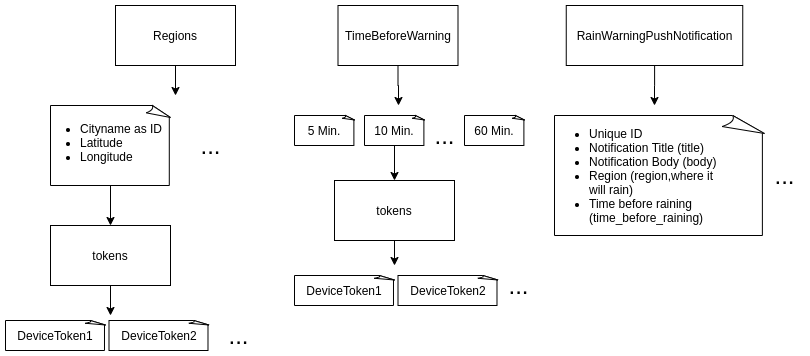
\includegraphics[width=0.6\textwidth,angle=0]{abb/datenbank_aufbau_uebersicht}
 \caption[Datenbankarchitektur]{Der Aufbau der Kollektionen und Dokumente in der Firebase}
\label{fig:datenbank_aufbau}
\end{figure}

\begin{sloppypar}
    \tolerance 9999
Jedes Gerät besitzt einen einmaligen Devicetoken welcher in zwei Kollektionen gespeichert wird. 
Die eine Kollektion steht für den Zeitpunkt, in dem die Regenwarnung gesendet werden soll, die andere Kollektion steht für die Region, in der die App verwendet wird. 
Diese beiden Kollektionen werden für das Senden der Push Benachrichtigungen benötigt, auf welches in dem Kapitel \ref{sec:Pushbenachrichtigungen} eingegangen wird. 
In den Einstellungen der App kann eingestellt wann die Regenwarnung als Push-Benachrichtigung gesendet werden soll.
Je nachdem, was der User einstellt, wird sein Devicetoken in eine andere Kollektion gespeichert. 
Dabei gibt es für jede einstellbare Zeit ein eigenes Dokument in der Kollektion TimeBeforeWarning. 
Wenn die Netze Regen vorhersagen, wird vom Server ein Dokument in RainWarningPushNotification gepusht. 
Dieses Dokument wird von einer Cloud-Function (Siehe Kapitel \ref{sec:Pushbenachrichtigungen}) verwendet, um die Pushbenachrichtigungen an die richtigen Geräte zu senden.
Der Cloud Storage von Firebase wird verwendet, um die PNGs mit der jeweiligen Vorhersage zu speichern.
Dabei lädt der Server alle 5 Minuten die neuen Vorhersagen hoch. Diese PNGs werden in der App angezeigt.
\end{sloppypar}